\documentclass{beamer}

\usetheme{Madrid}

\title{A Simple Beamer Knitr Example}
\author{Guy Yollin}

\usepackage{Sweave}
\begin{document}
\Sconcordance{concordance:te.tex:te.Rnw:%
1 7 1 1 0 7 1 1 2 1 0 2 1 6 0 1 2 3 1 1 7 2 0 2 1 3 0 1 5 7 1}


\maketitle

\begin{frame}[fragile]
\frametitle{Beamer slides can have code chucks}
Slides with code chunks need to be marked as "fragile"
\begin{Schunk}
\begin{Sinput}
> set.seed(1)
> x <- rnorm(100)
> mean(x)
\end{Sinput}
\begin{Soutput}
[1] 0.1088874
\end{Soutput}
\end{Schunk}
\end{frame}

\begin{frame}[fragile]
\frametitle{A graph from R}
\begin{Schunk}
\begin{Sinput}
> plot(cars$dist ~ cars$speed, pch = 16, 
+      col = 'orange', main = 'Distance vs Speed')
> library(gridGraphics)
> grid.echo()
\end{Sinput}
\end{Schunk}
\begin{center}
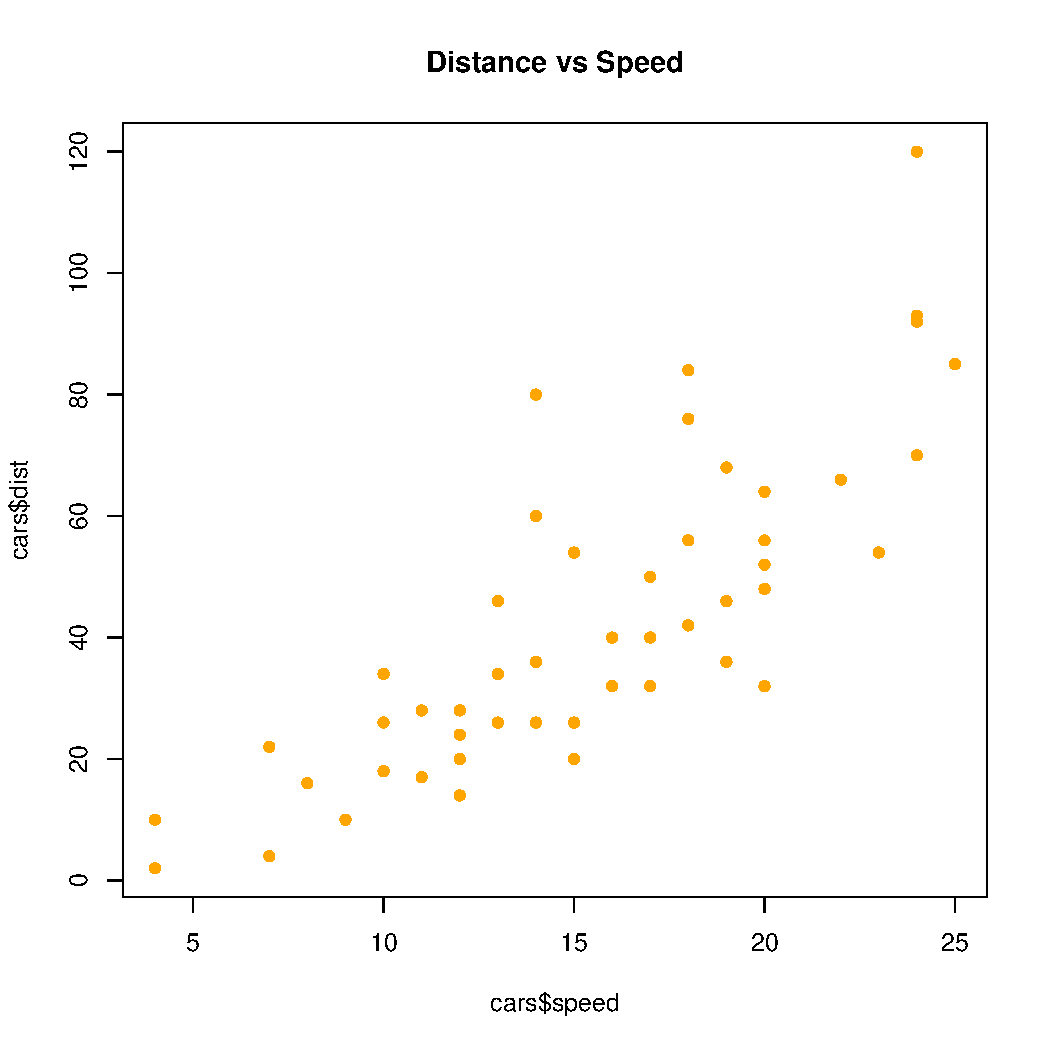
\includegraphics[height = 5.5cm, width = 5.5cm]{intro_1.pdf}
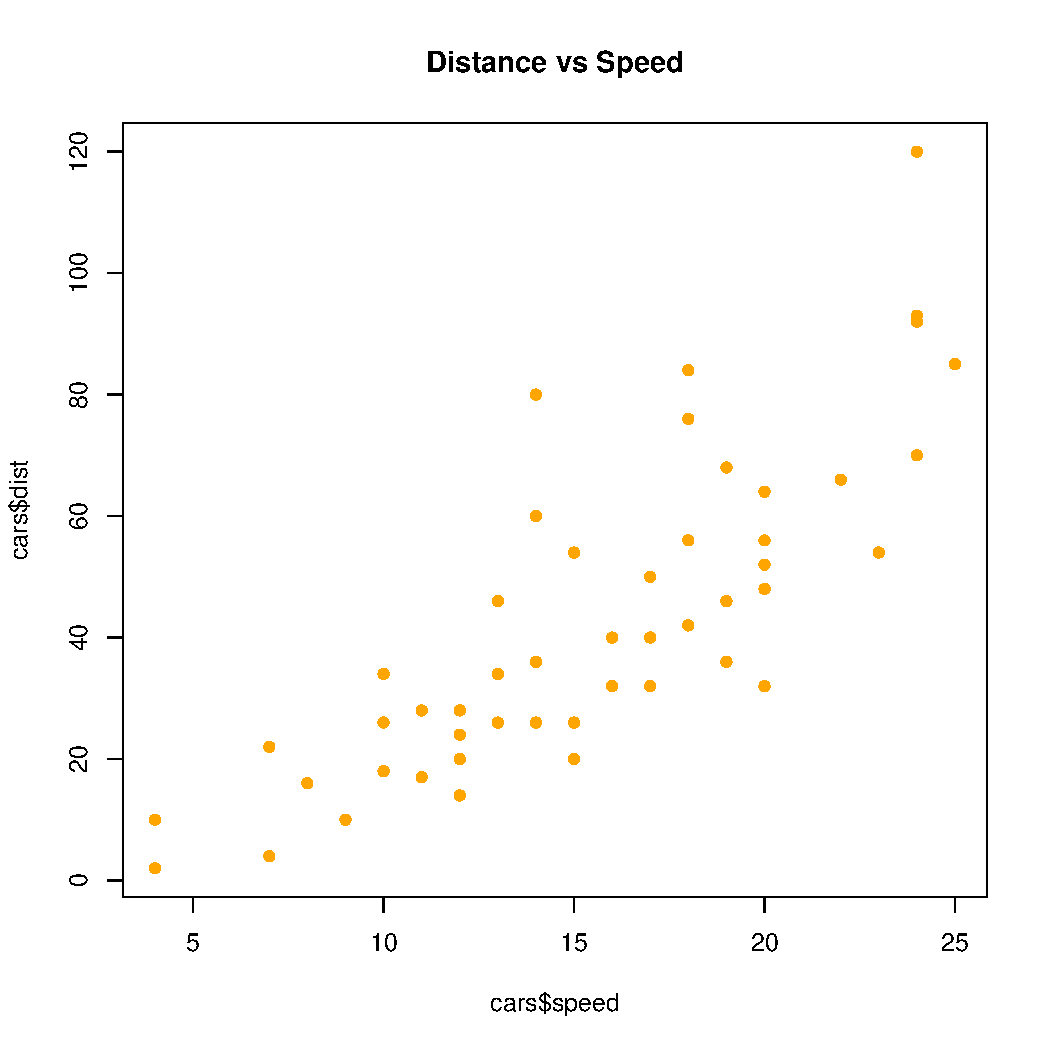
\includegraphics[height = 5.5cm, width = 5.5cm]{intro_2.pdf}
\end{center}

\end{frame}

\end{document}
